

\subsubsection{Cadre Général}


Ce module intervient après la phase d'analyse qui lui fourni, par l'intermédiaire de la mémoire, un ensemble d'environnements possibles et pour chacun d'eux un ensemble de formes reconnues. Le \og moteur de choix \fg{} se sert alors de la probabilité d'apparition des annotations associées aux formes reconnu afin d'évaluer chaque environnement possible. Il choisi finalement l'environnement qui maximise sa fonction objectif.

\subsubsection{Application aux jeux de plateau}


\begin{figure}[H] 
  \begin{center}
		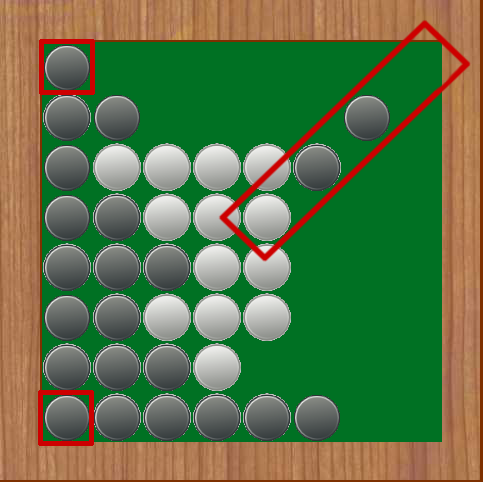
\includegraphics[width=0.3\textwidth]{files/raisonneur/moteur_de_choix} 
	\end{center}
\caption{Représentation graphique de l'environnement} 
\label{img_env}
\end{figure}
